\chapter{Introducción}

\section{Motivación}

\subsection{Antes de empezar...}

Antes de empezar a desarrollar una aplicación, debes saber que no será un camino sencillo, pero si muy gratificante. Cuando empecé a desarrollar la aplicación no sabía la cantidad de problemas a los que me iba a enfrentar, pero como tenía la ilusión de poder hacer realidad una idea todo fue más sencillo. 

\subsection{Classcity}

La idea de la que hablo se llama "Classcity" y consiste en una aplicación web cuya función principal es contactar profesores con alumnos para que puedan quedar y dar clases particulares de cualquier asignatura y curso. Esta idea nace porque llevo muchos años dedicándome a la enseñanza de clases particulares y pienso que hay una gran oportunidad de organizar mejorar la comunicación profesor-alumno. 

\subsection{M.E.A.N.}

Classcity ha sido desarrollada con 4 tecnologías diferentes que forman el famoso stack M.E.A.N. haciendo referencia a las siglas Mongo, Express, Angular y Node. Desde el cliente al servidor pasando por la base de datos, todas con el mismo punto en común. Desarrollo end-to-end usando JavaScript tanto en el frontend, backend y la base de datos. Sin entrar en definir complementamente cada una de las tecnologías que lo componen nos encontramos con:



\begin{itemize}

    \item MongoDB como base de datos que almacena documentos JSON.

    
    \item Express como web framework basado en Node.js que nos permite crear API REST, por ejemplo


    \item Angular como framework para crear la parte cliente de la aplicación en formato Single Page.

    
    \item Node.js como framework JavaScript basado en V8 que proporciona funcionalidades core para nuestra aplicación bajo un modelo asíncrono de eventos.
 
\end{itemize}


\subsection{Javascript}

MEAN como cualquier plataforma no puede vivir sin su comunidad, pero si tenemos en cuenta de que todas las tecnologías utilizan javascript como lenguaje de programación principal, podemos estar hablando de un stack bastante importante para la comunidad javascript, ya que todos los desarrolladores de front se podrán adentrar dentro del back y así poder hacer su propia aplicación.


\begin{figure}[H]
    \centering
    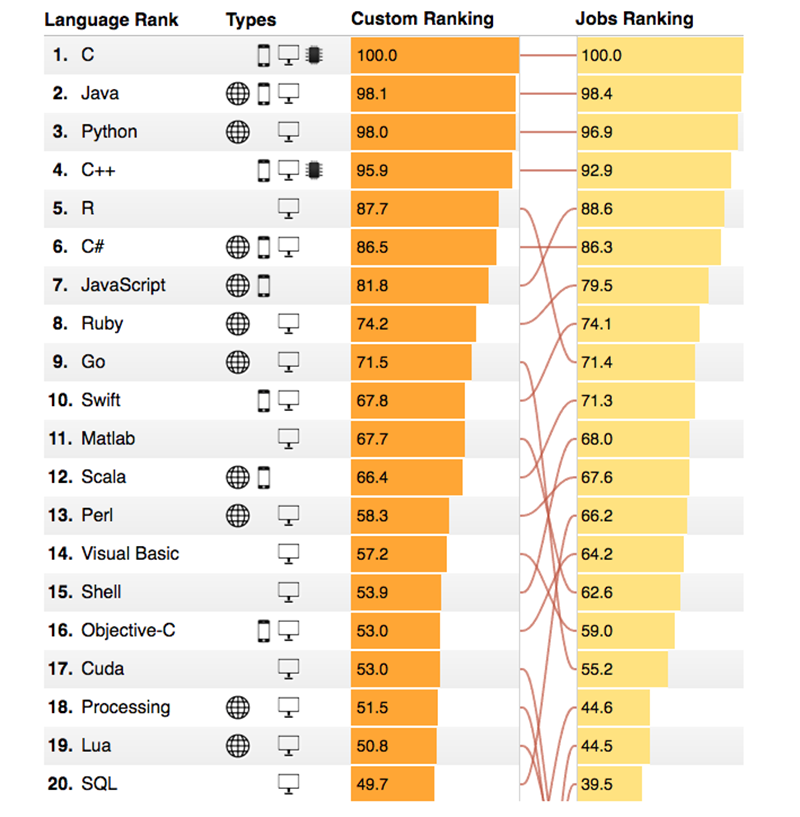
\includegraphics[width=60mm]{lenguajes.png}
\end{figure}

En este cuadro podemos encontrar información relevante de cómo están valorados los lenguajes de programación, en relación a la popularidad general de cada lenguaje de programación, pero también aplicando filtros por plataforma(computadores, móviles, web y sistemas embebidos) y por solicitud de empleo. Este estudio comenzó seleccionando unos 300 lenguajes en Github y escogiendo los más populares hasta quedarse con estos 20 candidatos para después estudiar la popularidad de esos lenguajes en 10 plataformas, que incluyen la propia Github, Google, Stack Overflow y paginas de oferta de empleo como Career Builder o Dice. 

Javascript a pesar de estar bien posicionado en el ranking tiene ventajas como que es un lenguaje muy sencillo y versátil, puesto que es muy útil para desarrollar páginas web y aplicaciones web. Otra cualidad que hace importante a javascript es su rapidez de computo, pudiendo ejecutar funciones inmediatamente, y por último y para mi la ventaja más importante es que es el único lenguaje que te permite trabajar modo FullStack en cualquier tipo de desarrollo de programación. Pero no todo puede ser buenas noticias para javascript, también tiene inconvenientes como por ejemplo que en el FrontEnd sus códigos son visibles, por lo tanto pueden ser leídos por cualquier usuario, y por otro lado javascrip también tiende a introducir gran cantidad de fragmentos de código en los sitios web.

\subsection{Plataforma Cloud}

También tengo que añadir la complejidad de subir una aplicación en la nube a través de la plataforma Amazon Web Service. Hay muchas otras plataforma de cloud como Azure(Microsoft), Google Cloud… Pero elegí AWS debido a que tiene un periodo de prueba gratuito y es bastante mas sencillo de manejar que Azure o Google Cloud. Además AWS es el líder indiscutible, aunque sus competidores últimamente alcanzan mas importancia en el mundo del cloud.

